
\documentclass{article}
\usepackage{amsfonts}
\usepackage{amsmath}

%%%%%%%%%%%%%%%%%%%%%%%%%%%%%%%%%%%%%%%%%%%%%%%%%%%%%%%%%%%%%%%%%%%%%%%%%%%%%%%%%%%%%%%%%%%%%%%%%%%%%%%%%%%%%%%%%%%%%%%%%%%%%%%%%%%%%%%%%%%%%%%%%%%%%%%%%%%%%%%%%%%%%%%%%%%%%%%%%%%%%%%%%%%%%%%%%%%%%%%%%%%%%
%TCIDATA{OutputFilter=LATEX.DLL}
%TCIDATA{Version=5.50.0.2960}
%TCIDATA{<META NAME="SaveForMode" CONTENT="1">}
%TCIDATA{BibliographyScheme=Manual}
%TCIDATA{Created=Tuesday, June 21, 2016 18:45:42}
%TCIDATA{LastRevised=Tuesday, June 21, 2016 23:05:16}
%TCIDATA{<META NAME="GraphicsSave" CONTENT="32">}
%TCIDATA{<META NAME="DocumentShell" CONTENT="Standard LaTeX\Blank - Standard LaTeX Article">}
%TCIDATA{CSTFile=40 LaTeX article.cst}

\newtheorem{theorem}{Theorem}
\newtheorem{acknowledgement}[theorem]{Acknowledgement}
\newtheorem{algorithm}[theorem]{Algorithm}
\newtheorem{axiom}[theorem]{Axiom}
\newtheorem{case}[theorem]{Case}
\newtheorem{claim}[theorem]{Claim}
\newtheorem{conclusion}[theorem]{Conclusion}
\newtheorem{condition}[theorem]{Condition}
\newtheorem{conjecture}[theorem]{Conjecture}
\newtheorem{corollary}[theorem]{Corollary}
\newtheorem{criterion}[theorem]{Criterion}
\newtheorem{definition}[theorem]{Definition}
\newtheorem{example}[theorem]{Example}
\newtheorem{exercise}[theorem]{Exercise}
\newtheorem{lemma}[theorem]{Lemma}
\newtheorem{notation}[theorem]{Notation}
\newtheorem{problem}[theorem]{Problem}
\newtheorem{proposition}[theorem]{Proposition}
\newtheorem{remark}[theorem]{Remark}
\newtheorem{solution}[theorem]{Solution}
\newtheorem{summary}[theorem]{Summary}
\newenvironment{proof}[1][Proof]{\noindent\textbf{#1.} }{\ \rule{0.5em}{0.5em}}
\input{tcilatex}

\begin{document}


\section{Empirical Analysis}

As mentioned in the introduction, we argue that in equilibrium the large
trader is statistically indistinguishable from an atomistic trader. The
clearing price $\pi (t)$ on the exchange will thus be%
\[
\pi (t)\equiv P(0,t)
\]

so that $Q(\pi (t),t)=0$. In this section, we calibrate the market model and
then simulate it in the risk-neutral measure to price options. We use
empirical high frequency data of a magnitude of a millisecond. Then the
calibrated parameters are utilized in the discretized simulation model in
both the physical and risk-neutral measures. When simulating the net demand
curve $Q$ in the risk neutral measure, the market price of risk equation is
solved. As expected, we could not find any case where the market price of
risk equation does not have a solution.

\subsection{Data}

The high frequency trading data are collected from the NYSE Arcabook limit
orders for April 2011. Historical NYSE Arcabook data provide information of
the complete limit order book (LOB) from NYSE, NYSE Arca, NYSE MKT, NASDAQ
and the ArcaEdge platforms from 3:30 a.m. to 8:00 p.m. ET under high speed
of latencies (less than 5 milliseconds). Each limit order contains the
unique reference number, the time stamp in seconds and milliseconds, the
limit price in U.S. dollars, the quantity in number of shares, and the
trading type (\textquotedblleft B\textquotedblright : buy or
\textquotedblleft S\textquotedblright :sell).

All the limit order book records are categorized into three groups:
\textquotedblright A\textquotedblright\ Add, \textquotedblright
M\textquotedblright\ Modified and \textquotedblright D\textquotedblright\
Deleted. For the market liquidity model, we consider the net demand of the
stock, which is captured by summing added records (\textquotedblright
A\textquotedblright ) with modified (\textquotedblright M\textquotedblright
) adjustment and subtracting the deleted orders. To be specific, within a
certain partitioned time period, the added orders would be updated by the
modified orders, if applicable and the orders occur in the same partitioned
period.

In this section, we use the time series  of Apple Inc. stock (AAPL) as of
April 1st 2011 for calibration.

\bigskip

\subsection{Discretized Model}

The price variable $p$ belongs to the set $\{0,\Delta p,2\Delta p,..,I\Delta
p\}$ where $I=401$ and $\Delta p=\$1.91$. This corresponds for our data set
to a winsorization at the 99\% quantile of the price for all the limit
orders within the trading day. The variable $s$ will belong to the same set,
so we set $\Delta s=\Delta p$. The variable $t$ will be a multiple of $%
\Delta t$, for $\Delta t$=15 minutes. For any function $f$ of real-valued
variables $p=k\Delta p,$ $s=i\Delta s$ and $t=j\Delta t$ we streamline the
notation by writing:
\begin{eqnarray*}
f(k,i,j) &\leftarrow &f(k\Delta p,i\Delta s,j\Delta t) \\
\Delta f(k,i,j) &=&f(k,i,j+1)-f(k,i,j)
\end{eqnarray*}
We denote observed quantities by $\hat{f}(t)$ and simulated quantities by $%
f(t)$. We discretize the model (\ref{equ_h_A}) to (\ref{equ_Q_A}), and
simplify it by setting most of the drifts equal to zero.  Let $\{z(i,j)\}$
be a collection of standard normal random variates where $0\leq i\leq I$,
and the values of $j$ will be clear from context. After initializing all
stochastic processes, we use the Euler scheme:%
\begin{eqnarray}
\Delta h(k,j) &=&\sigma _{h}(k)\sum_{i=2}^{I}b_{h}(k,i)z(i,j)\sqrt{\Delta
s\Delta t}\text{ \ \ \ }2\leq k\leq I  \label{Euler_1} \\
\Delta q(1,j) &=&\sigma _{q}(1)\sum_{i=2}^{I}b_{q}(1,i)z(i,j)\sqrt{\Delta
s\Delta t}  \label{Euler_2} \\
\Delta \eta (j) &=&a_{\eta }(\bar{\eta}-\eta (j))\Delta t+\sigma _{\eta }%
\sqrt{\eta (j)(1-\eta (j))}\sum_{i=0}^{I}b_{\eta }(i)z(i,j)\sqrt{\Delta
s\Delta t}  \label{Euler_3}
\end{eqnarray}

We then complete the model by setting, for \ $2\leq k\leq I$:%
\begin{eqnarray*}
q(k,j) &=&q(1,j)\exp \left( {\sum_{i=2}^{k}h(i,j)\Delta p}\right) \text{ \ \
} \\
Q(0,j) &=&\frac{\eta (j)}{2-\eta (j)}\sum_{i=1}^{I}q(i,j){\Delta p} \\
Q(k,j) &=&[Q(0,j)+\sum_{i=1}^{I}q(i,j)\Delta p]\eta
(j)-[Q(0,j)+\sum_{i=1}^{k}q(i,j)\Delta p]
\end{eqnarray*}

\subsection{Calibration Methodology}

The number of observations is equal to $N=32$. Observation times take values
in the set $\{-N\Delta t,-(N-1)\Delta t,..,0\}$. Since each time step
represents an interval of 15 minutes. we use all the dates between April 1st
9 AM and April 1st 5PM, which covers the regular trading hours during the
day. The net demand $Q$ at price $p$  is calculated, by definition as:

\begin{gather*}
\hat{Q}(k,.)=\text{quantity of shares available for purchase at a price }>k{%
\Delta p} \\
\text{ \ \ \ \ \ \ \ \ \ }-\text{quantity of shares available for sale at a
price }<k{\Delta p}
\end{gather*}

A typical net demand $\hat{Q}$ surface as a function of price and time for
AAPL stock on April 1st, 2011 is shown in %Figure~\ref{fig::AAPL_20110401_Calibration_Q}.

\begin{center}
\begin{figure}[tbp]
\centering
% Requires \usepackage{graphicx}
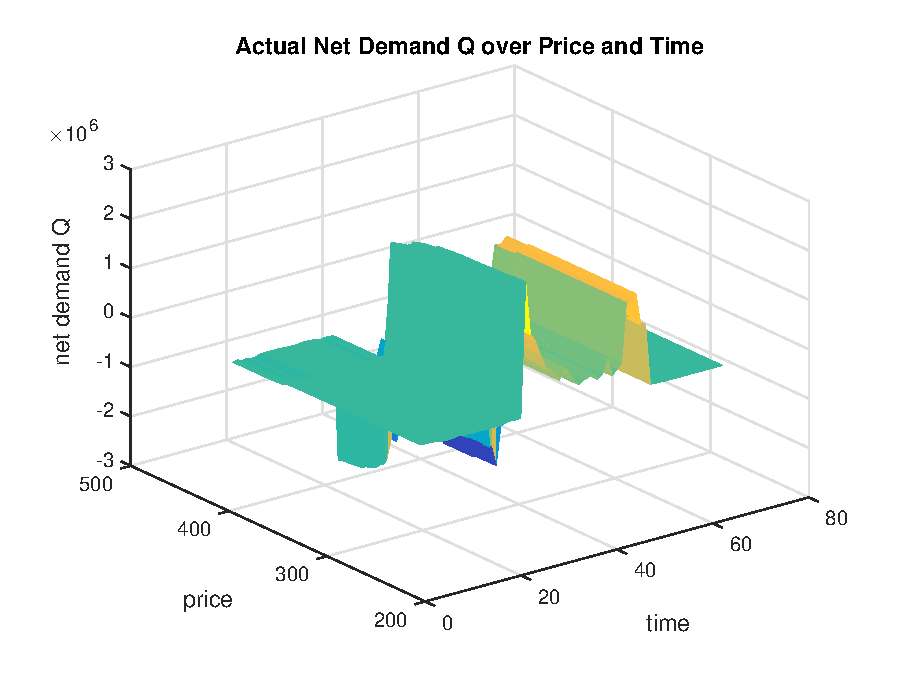
\includegraphics[scale = 0.7]{AAPL_20110401_Calibration_Q.eps}\newline
\caption{The calculated net demand surface $Q$ by price and time, from
market data for AAPL as of April 1st, 2011.}
\label{fig::AAPL_20110401_Calibration_Q}
\end{figure}
\end{center}

After the net demand surface $\hat{Q}$ is calculated, the net demand density
$\hat{q}$ is calculated by taking the first order difference of $\hat{Q}(p)$:

\[
\hat{q}(k,j)=-\frac{\hat{Q}(k,j)-\hat{Q}(k-1,j)}{\Delta p}\text{, \ \  \ \ \
}1\leq k\leq I
\]

Discretization of (\ref{equ_q_A}) yields:%
\[
\hat{h}(k,j)=\frac{1}{\Delta p}(\log (\hat{q}(k,j))-\log {\hat{q}(k-1,j)),}%
\text{ \ \  \ \ \ }2\leq k\leq I
\]%
The net demand elasticity $\hat{\eta}$ is calculated by (\ref{eta}). We
estimate the instantaneous variances by the method of moments:
\begin{eqnarray*}
\hat{\sigma}_{\eta }^{2} &=&\frac{1}{N\Delta t}\sum_{j=-N}^{-1}\frac{\Delta
\hat{\eta}(j)^{2}}{\hat{\eta}(j)(1-\hat{\eta}(j))} \\
\hat{\sigma}_{q}^{2}(1) &=&\frac{1}{N\Delta t}\sum_{j=-N}^{-1}\Delta \hat{q}%
(1,j)^{2} \\
\hat{\sigma}_{h}^{2}(k) &=&\frac{1}{N\Delta t}\sum_{j=-N}^{-1}\Delta \hat{h}%
(k,j)^{2}\text{\ \ \ \ \ \ \ \ \ \ }k=2,...,S
\end{eqnarray*}

We do the same for the instantaneous covariances:%
\begin{eqnarray*}
\hat{s}_{\eta ,q}^{2}(1) &=&\frac{1}{N\Delta t}\sum_{j=-N}^{-1}\Delta \hat{%
\eta}(j)\Delta \hat{q}(1,j) \\
\hat{s}_{\eta ,h}^{2}(k) &=&\frac{1}{N\Delta t}\sum_{j=-N}^{-1}\frac{\Delta
\hat{\eta}(j)\Delta \hat{h}(k,j)}{\sqrt{\eta (j)(1-\eta (j))}}\text{ \ \ \ \
\ \ \ \ \ \ }k=2,...,S \\
\hat{s}_{q,h}^{2}(1,k) &=&\frac{1}{N\Delta t}\sum_{j=-N}^{-1}\Delta \hat{q}%
(1,j)\Delta \hat{h}(k,j)\text{ \ \ \ \ \ \ \ \ \ \ \ \ \ \ \ \ \ }k=2,...,S
\\
\hat{s}_{h}^{2}(k_{1},k_{2}) &=&\frac{1}{N\Delta t}\sum_{j=-N}^{-1}\Delta
\hat{h}(k_{1},j)\Delta \hat{h}(k_{2},j)\text{ \ \ \ \ \ \ \ \ \ \ \ \ \ \ \
\ \ }k_{1},k_{2}=2,...,S
\end{eqnarray*}

We organize the instantaneous variance-covariance matrix as:%
\[
V=\left(
\begin{array}{ccccc}
\hat{\sigma}_{\eta }^{2} & \hat{s}_{\eta ,q}^{2}(1) & \hat{s}_{\eta
,h}^{2}(2) &  & \hat{s}_{\eta ,h}^{2}(I) \\
\hat{s}_{\eta ,q}^{2}(1) & \hat{\sigma}_{q}^{2}(1) & \hat{s}_{q,h}^{2}(1,2)
& \cdots  & \hat{s}_{q_{,}h}^{2}(1,I) \\
\hat{s}_{\eta ,h}^{2}(2) & \hat{s}_{q,h}^{2}(1,2) & \hat{\sigma}_{h}^{2}(2)
& \cdots  & \hat{s}_{h}^{2}(2,I) \\
\vdots  & \vdots  & \vdots  & \ddots  & \vdots  \\
\hat{s}_{\eta ,h}^{2}(I) & \hat{s}_{q_{,}h}^{2}(1,I) & \hat{s}_{h}^{2}(2,I)
& \cdots  & \hat{\sigma}_{h}^{2}(I)%
\end{array}%
\right)
\]%
The factor loading matrix $B$ is the square root of the correlation matrix
corresponding to $V$. It is made of the following coefficients:%
\[
\hat{B}=\left(
\begin{array}{ccccc}
\hat{b}_{\eta }(0) & 0 & \cdots  & \cdots  & \cdots  \\
\hat{b}_{\eta }(1) & \hat{b}_{q}(1,1) & \ddots  &  & \vdots  \\
& \vdots  & \hat{b}_{h}(2,1) & \ddots  & \vdots  \\
& \vdots  & \vdots  & \ddots  & 0 \\
\hat{b}_{\eta }(I) & \hat{b}_{q}(1,I) & \hat{b}_{h}(I,1) & \cdots  & \hat{b}%
_{h}(I,I)%
\end{array}%
\right)
\]

We use Cholesky decomposition to calculate $\hat{B}.$

\bigskip

RAN:\ please provide the values for $a_{\eta }$ and$\ \bar{\eta}$ (no
justification needed).

\subsection{Simulation - Real-world Measure ($\mathbb{P}$ Measure)}

The simulated net demand curve under physical measure using the above
methods is shown in left graph of Figure~\ref%
{fig::AAPL_20110401_simulated_both_measures}.

\begin{center}
\begin{figure}[tbp]
\centering
% Requires \usepackage{graphicx}
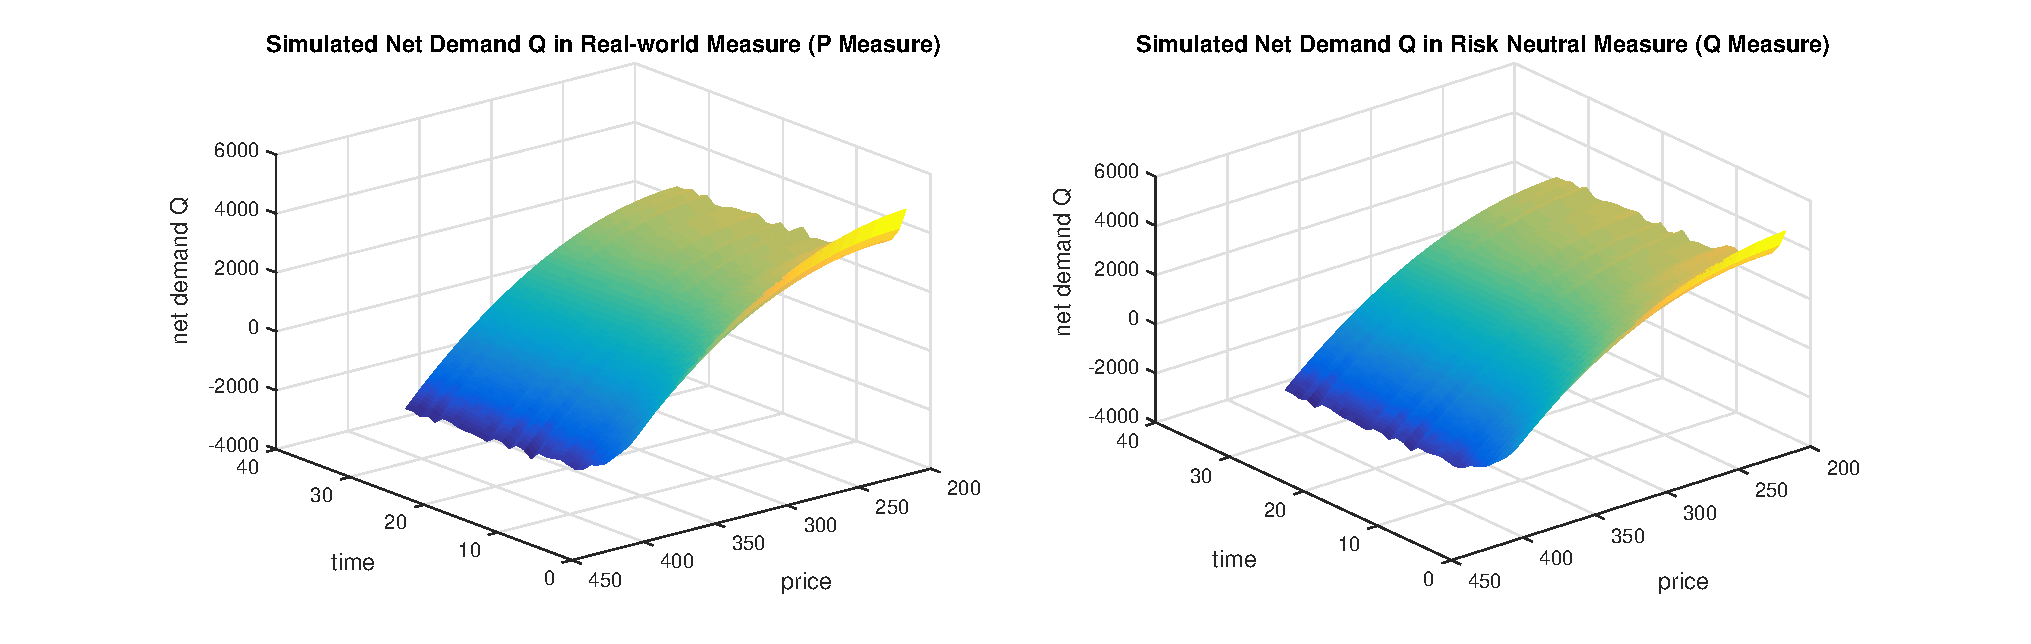
\includegraphics[scale = 0.5]{Q_both_measures.eps}\newline
\caption{The simulated net demand surface Q(p,t) under physical measure
(left) and risk neutral measure (right).}
\label{fig::AAPL_20110401_simulated_Q_P_measure}
\end{figure}
\end{center}

\subsection{Simulation - Risk-Neutral Measure ($\mathbb{Q}$ Measure)}

Let $k^{\ast }(j)$ be the index of the approximate clearing price, i.e., the
value of $k$ that minimizes $|Q(k,j)|$.

We first need to solve the market price of risk equations. Expressions for $%
\mu _{Q}(k,j)$ and $\sigma _{Q}(k,j)$ and $b_{Q}(k,i,j)$ are obtained by
discretization of equations 41 and 42 in the appendix (Ran, please make the
exact reference). Details are left to the reader. Remember (Ran find the
exact reference) that:

\[
\Sigma _{Q}(k,i,j)=\sigma _{Q}(k,j)b_{Q}(k,i,j)
\]

We calculate:

\begin{eqnarray*}
\sigma _{\pi }(j)b_{\pi }(i,j) &=&-\frac{\Sigma _{Q}(k^{\ast }(j),i,j)}{%
q(k^{\ast }(j),j)} \\
C(k,j) &=&\sigma _{\pi }(j)\sum_{i=0}^{I}\frac{\Sigma _{Q}(k^{\ast
}(j),i,j)-\Sigma _{Q}(k^{\ast }(j)-1,i,j)}{\Delta p}b_{\pi }(i,j) \\
B(k,j) &=&\mu _{Q}(k,j)-\frac{1}{2}\frac{Q(k+1,j)-2Q(k,j)+Q(k-1,j)}{\Delta
p^{2}}+C(k,j)
\end{eqnarray*}

The market price of risk equations are, for each scenario and each time $j$:

\[
\sum_{i=0}^{I}\Sigma _{Q}(k,i,j)\lambda (i,j)=B(k,j)\text{ \ \ \ }k=0,...,I
\]

Now let $\{z^{\mathbb{Q}}(i,j)\}$ be a collection of standard normal random
variates. It remains only to make the substitution:

\[
z(i,j)=z^{\mathbb{Q}}(i,j)\sqrt{\Delta t\Delta s}-\lambda (i,j)\sqrt{\Delta s%
}
\]

in our model (\ref{Euler_1})\ to (\ref{Euler_3}) to obtain the risk-neutral
model.

The simulated net demand curve under risk neutral measure is shown in the
right graph of Figure~\ref{fig::AAPL_20110401_simulated_both_measures}. The
range of the difference (Ran:\ of what? a $\mathbb{P}$-measure simulation is
not a number!!\} between $\mathbb{P}$-measure simulation and $\mathbb{Q}$%
-measure simulation is $[-50.22,66.10]$ in the case shown in the simulation.

\end{document}
